\documentclass[1p]{elsarticle_modified}
%\bibliographystyle{elsarticle-num}

%\usepackage[colorlinks]{hyperref}
%\usepackage{abbrmath_seonhwa} %\Abb, \Ascr, \Acal ,\Abf, \Afrak
\usepackage{amsfonts}
\usepackage{amssymb}
\usepackage{amsmath}
\usepackage{amsthm}
\usepackage{scalefnt}
\usepackage{amsbsy}
\usepackage{kotex}
\usepackage{caption}
\usepackage{subfig}
\usepackage{color}
\usepackage{graphicx}
\usepackage{xcolor} %% white, black, red, green, blue, cyan, magenta, yellow
\usepackage{float}
\usepackage{setspace}
\usepackage{hyperref}

\usepackage{tikz}
\usetikzlibrary{arrows}

\usepackage{multirow}
\usepackage{array} % fixed length table
\usepackage{hhline}

%%%%%%%%%%%%%%%%%%%%%
\makeatletter
\renewcommand*\env@matrix[1][\arraystretch]{%
	\edef\arraystretch{#1}%
	\hskip -\arraycolsep
	\let\@ifnextchar\new@ifnextchar
	\array{*\c@MaxMatrixCols c}}
\makeatother %https://tex.stackexchange.com/questions/14071/how-can-i-increase-the-line-spacing-in-a-matrix
%%%%%%%%%%%%%%%

\usepackage[normalem]{ulem}

\newcommand{\msout}[1]{\ifmmode\text{\sout{\ensuremath{#1}}}\else\sout{#1}\fi}
%SOURCE: \msout is \stkout macro in https://tex.stackexchange.com/questions/20609/strikeout-in-math-mode

\newcommand{\cancel}[1]{
	\ifmmode
	{\color{red}\msout{#1}}
	\else
	{\color{red}\sout{#1}}
	\fi
}

\newcommand{\add}[1]{
	{\color{blue}\uwave{#1}}
}

\newcommand{\replace}[2]{
	\ifmmode
	{\color{red}\msout{#1}}{\color{blue}\uwave{#2}}
	\else
	{\color{red}\sout{#1}}{\color{blue}\uwave{#2}}
	\fi
}

\newcommand{\Sol}{\mathcal{S}} %segment
\newcommand{\D}{D} %diagram
\newcommand{\A}{\mathcal{A}} %arc


%%%%%%%%%%%%%%%%%%%%%%%%%%%%%5 test

\def\sl{\operatorname{\textup{SL}}(2,\Cbb)}
\def\psl{\operatorname{\textup{PSL}}(2,\Cbb)}
\def\quan{\mkern 1mu \triangleright \mkern 1mu}

\theoremstyle{definition}
\newtheorem{thm}{Theorem}[section]
\newtheorem{prop}[thm]{Proposition}
\newtheorem{lem}[thm]{Lemma}
\newtheorem{ques}[thm]{Question}
\newtheorem{cor}[thm]{Corollary}
\newtheorem{defn}[thm]{Definition}
\newtheorem{exam}[thm]{Example}
\newtheorem{rmk}[thm]{Remark}
\newtheorem{alg}[thm]{Algorithm}

\newcommand{\I}{\sqrt{-1}}
\begin{document}

%\begin{frontmatter}
%
%\title{Boundary parabolic representations of knots up to 8 crossings}
%
%%% Group authors per affiliation:
%\author{Yunhi Cho} 
%\address{Department of Mathematics, University of Seoul, Seoul, Korea}
%\ead{yhcho@uos.ac.kr}
%
%
%\author{Seonhwa Kim} %\fnref{s_kim}}
%\address{Center for Geometry and Physics, Institute for Basic Science, Pohang, 37673, Korea}
%\ead{ryeona17@ibs.re.kr}
%
%\author{Hyuk Kim}
%\address{Department of Mathematical Sciences, Seoul National University, Seoul 08826, Korea}
%\ead{hyukkim@snu.ac.kr}
%
%\author{Seokbeom Yoon}
%\address{Department of Mathematical Sciences, Seoul National University, Seoul, 08826,  Korea}
%\ead{sbyoon15@snu.ac.kr}
%
%\begin{abstract}
%We find all boundary parabolic representation of knots up to 8 crossings.
%
%\end{abstract}
%\begin{keyword}
%    \MSC[2010] 57M25 
%\end{keyword}
%
%\end{frontmatter}

%\linenumbers
%\tableofcontents
%
\newcommand\colored[1]{\textcolor{white}{\rule[-0.35ex]{0.8em}{1.4ex}}\kern-0.8em\color{red} #1}%
%\newcommand\colored[1]{\textcolor{white}{ #1}\kern-2.17ex	\textcolor{white}{ #1}\kern-1.81ex	\textcolor{white}{ #1}\kern-2.15ex\color{red}#1	}

{\Large $\underline{11a_{207}~(K11a_{207})}$}

\setlength{\tabcolsep}{10pt}
\renewcommand{\arraystretch}{1.6}
\vspace{1cm}\begin{tabular}{m{100pt}>{\centering\arraybackslash}m{274pt}}
\multirow{5}{120pt}{
	\centering
	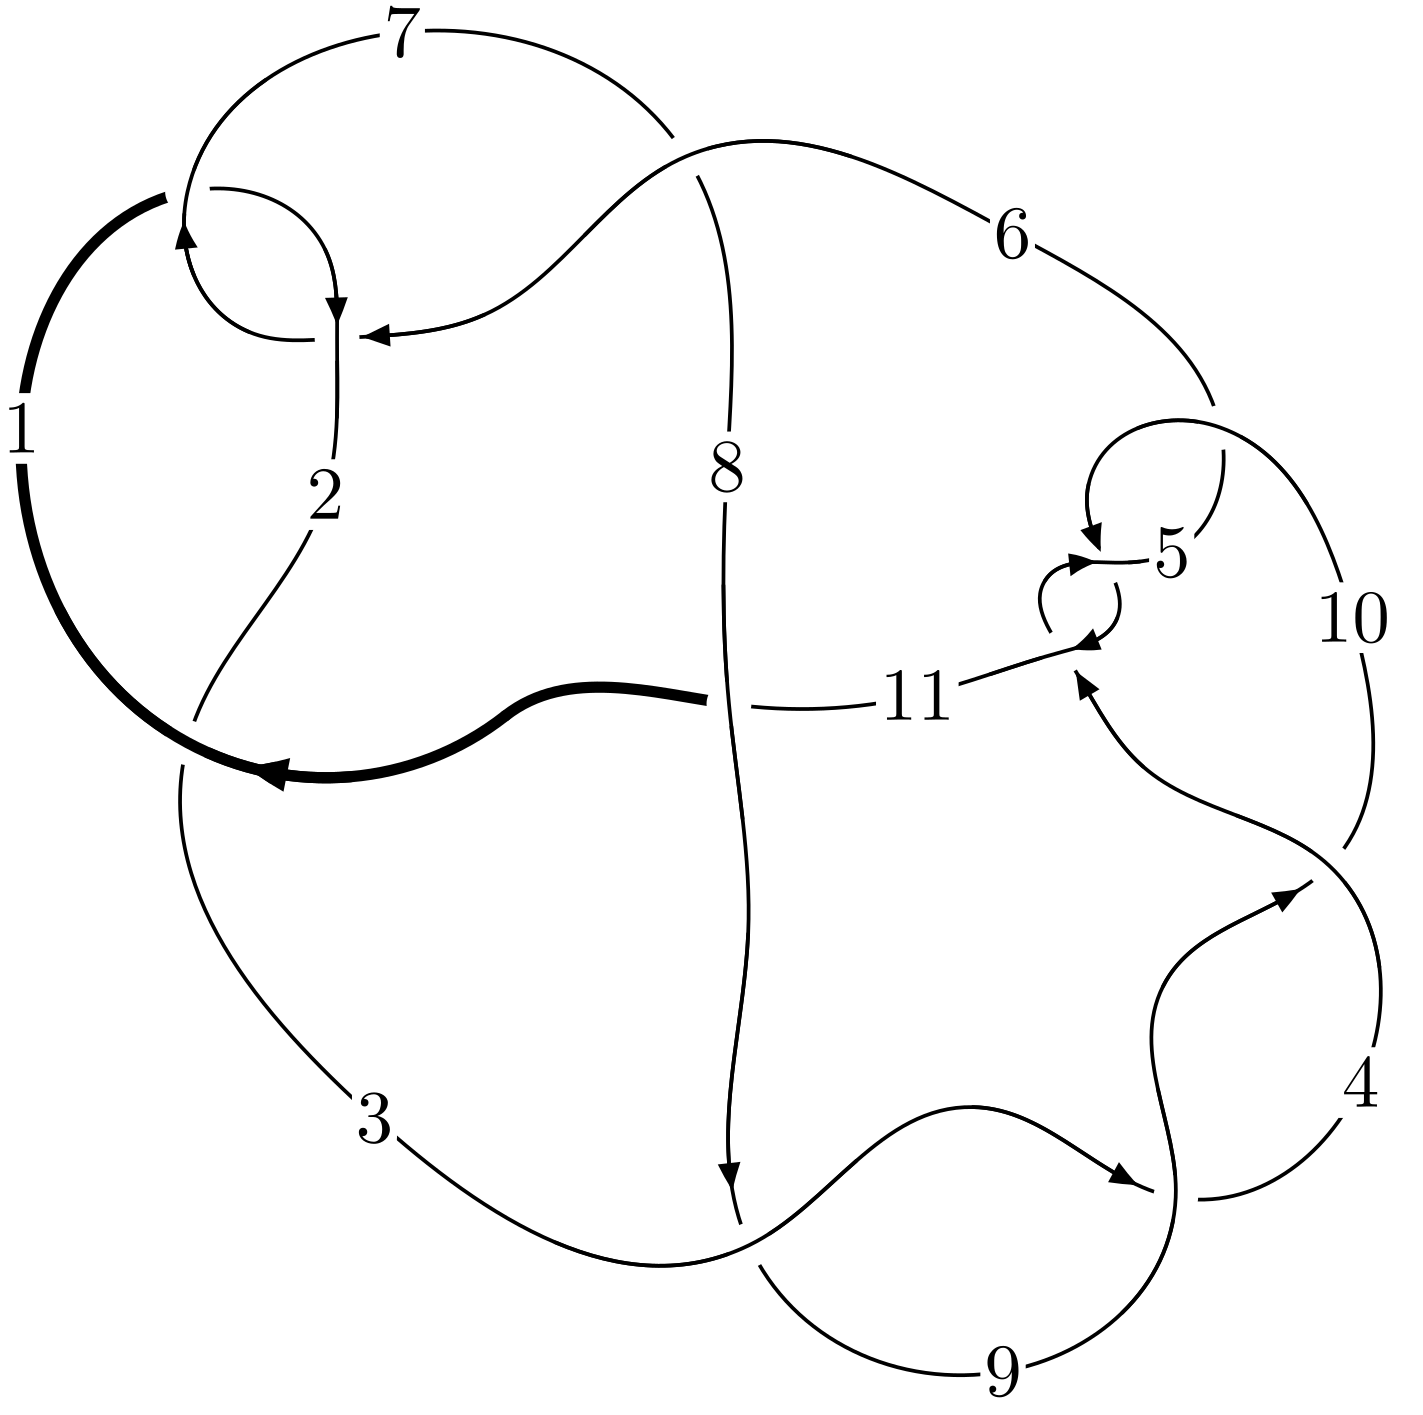
\includegraphics[width=112pt]{../../../GIT/diagram.site/Diagrams/png/456_11a_207.png}\\
\ \ \ A knot diagram\footnotemark}&
\allowdisplaybreaks
\textbf{Linearized knot diagam} \\
\cline{2-2}
 &
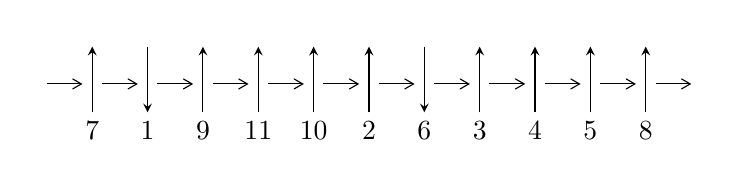
\begin{tikzpicture}[x=20pt, y=17pt]
	% nodes
	\node (C0) at (0, 0) {};
	\node (C1) at (1, 0) {};
	\node (C1U) at (1, +1) {};
	\node (C1D) at (1, -1) {7};

	\node (C2) at (2, 0) {};
	\node (C2U) at (2, +1) {};
	\node (C2D) at (2, -1) {1};

	\node (C3) at (3, 0) {};
	\node (C3U) at (3, +1) {};
	\node (C3D) at (3, -1) {9};

	\node (C4) at (4, 0) {};
	\node (C4U) at (4, +1) {};
	\node (C4D) at (4, -1) {11};

	\node (C5) at (5, 0) {};
	\node (C5U) at (5, +1) {};
	\node (C5D) at (5, -1) {10};

	\node (C6) at (6, 0) {};
	\node (C6U) at (6, +1) {};
	\node (C6D) at (6, -1) {2};

	\node (C7) at (7, 0) {};
	\node (C7U) at (7, +1) {};
	\node (C7D) at (7, -1) {6};

	\node (C8) at (8, 0) {};
	\node (C8U) at (8, +1) {};
	\node (C8D) at (8, -1) {3};

	\node (C9) at (9, 0) {};
	\node (C9U) at (9, +1) {};
	\node (C9D) at (9, -1) {4};

	\node (C10) at (10, 0) {};
	\node (C10U) at (10, +1) {};
	\node (C10D) at (10, -1) {5};

	\node (C11) at (11, 0) {};
	\node (C11U) at (11, +1) {};
	\node (C11D) at (11, -1) {8};
	\node (C12) at (12, 0) {};

	% arrows
	\draw[->,>={angle 60}]
	(C0) edge (C1) (C1) edge (C2) (C2) edge (C3) (C3) edge (C4) (C4) edge (C5) (C5) edge (C6) (C6) edge (C7) (C7) edge (C8) (C8) edge (C9) (C9) edge (C10) (C10) edge (C11) (C11) edge (C12) ;	\draw[->,>=stealth]
	(C1D) edge (C1U) (C2U) edge (C2D) (C3D) edge (C3U) (C4D) edge (C4U) (C5D) edge (C5U) (C6D) edge (C6U) (C7U) edge (C7D) (C8D) edge (C8U) (C9D) edge (C9U) (C10D) edge (C10U) (C11D) edge (C11U) ;
	\end{tikzpicture} \\
\hhline{~~} \\& 
\textbf{Solving Sequence} \\ \cline{2-2} 
 &
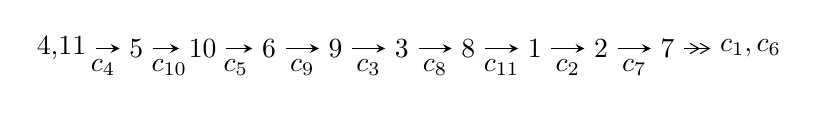
\begin{tikzpicture}[x=24pt, y=7pt]
	% node
	\node (A0) at (-1/8, 0) {4,11};
	\node (A1) at (1, 0) {5};
	\node (A2) at (2, 0) {10};
	\node (A3) at (3, 0) {6};
	\node (A4) at (4, 0) {9};
	\node (A5) at (5, 0) {3};
	\node (A6) at (6, 0) {8};
	\node (A7) at (7, 0) {1};
	\node (A8) at (8, 0) {2};
	\node (A9) at (9, 0) {7};
	\node (C1) at (1/2, -1) {$c_{4}$};
	\node (C2) at (3/2, -1) {$c_{10}$};
	\node (C3) at (5/2, -1) {$c_{5}$};
	\node (C4) at (7/2, -1) {$c_{9}$};
	\node (C5) at (9/2, -1) {$c_{3}$};
	\node (C6) at (11/2, -1) {$c_{8}$};
	\node (C7) at (13/2, -1) {$c_{11}$};
	\node (C8) at (15/2, -1) {$c_{2}$};
	\node (C9) at (17/2, -1) {$c_{7}$};
	\node (A10) at (41/4, 0) {$c_{1},c_{6}$};

	% edge
	\draw[->,>=stealth]	
	(A0) edge (A1) (A1) edge (A2) (A2) edge (A3) (A3) edge (A4) (A4) edge (A5) (A5) edge (A6) (A6) edge (A7) (A7) edge (A8) (A8) edge (A9) ;
	\draw[->>,>={angle 60}]	
	(A9) edge (A10);
\end{tikzpicture} \\ 

\end{tabular} \\

\footnotetext{
The image of knot diagram is generated by the software ``\textbf{Draw programme}" developed by Andrew Bartholomew(\url{http://www.layer8.co.uk/maths/draw/index.htm\#Running-draw}), where we modified some parts for our purpose(\url{https://github.com/CATsTAILs/LinksPainter}).
}\phantom \\ \newline 
\centering \textbf{Ideals for irreducible components\footnotemark of $X_{\text{par}}$} 
 
\begin{align*}
I^u_{1}&=\langle 
u^{42}+u^{41}+\cdots- u-1\rangle \\
\\
\end{align*}
\raggedright * 1 irreducible components of $\dim_{\mathbb{C}}=0$, with total 42 representations.\\
\footnotetext{All coefficients of polynomials are rational numbers. But the coefficients are sometimes approximated in decimal forms when there is not enough margin.}
\newpage
\renewcommand{\arraystretch}{1}
\centering \section*{I. $I^u_{1}= \langle u^{42}+u^{41}+\cdots- u-1 \rangle$}
\flushleft \textbf{(i) Arc colorings}\\
\begin{tabular}{m{7pt} m{180pt} m{7pt} m{180pt} }
\flushright $a_{4}=$&$\begin{pmatrix}1\\0\end{pmatrix}$ \\
\flushright $a_{11}=$&$\begin{pmatrix}0\\u\end{pmatrix}$ \\
\flushright $a_{5}=$&$\begin{pmatrix}1\\- u^2\end{pmatrix}$ \\
\flushright $a_{10}=$&$\begin{pmatrix}- u\\u^3+u\end{pmatrix}$ \\
\flushright $a_{6}=$&$\begin{pmatrix}u^2+1\\- u^4-2 u^2\end{pmatrix}$ \\
\flushright $a_{9}=$&$\begin{pmatrix}- u^3-2 u\\u^3+u\end{pmatrix}$ \\
\flushright $a_{3}=$&$\begin{pmatrix}- u^6-3 u^4-2 u^2+1\\u^6+2 u^4+u^2\end{pmatrix}$ \\
\flushright $a_{8}=$&$\begin{pmatrix}u^9+4 u^7+5 u^5-3 u\\- u^9-3 u^7-3 u^5+u\end{pmatrix}$ \\
\flushright $a_{1}=$&$\begin{pmatrix}u^{19}+8 u^{17}+26 u^{15}+40 u^{13}+19 u^{11}-24 u^9-30 u^7+9 u^3\\- u^{19}-7 u^{17}-20 u^{15}-27 u^{13}-11 u^{11}+13 u^9+14 u^7-3 u^3+u\end{pmatrix}$ \\
\flushright $a_{2}=$&$\begin{pmatrix}- u^{32}-13 u^{30}+\cdots-2 u^2+1\\u^{32}+12 u^{30}+\cdots-8 u^6+10 u^4\end{pmatrix}$ \\
\flushright $a_{7}=$&$\begin{pmatrix}u^{15}+6 u^{13}+14 u^{11}+14 u^9+2 u^7-6 u^5-4 u^3-2 u\\- u^{17}-7 u^{15}-19 u^{13}-22 u^{11}-3 u^9+14 u^7+6 u^5-2 u^3+u\end{pmatrix}$\\ \flushright $a_{7}=$&$\begin{pmatrix}u^{15}+6 u^{13}+14 u^{11}+14 u^9+2 u^7-6 u^5-4 u^3-2 u\\- u^{17}-7 u^{15}-19 u^{13}-22 u^{11}-3 u^9+14 u^7+6 u^5-2 u^3+u\end{pmatrix}$\\&\end{tabular}
\flushleft \textbf{(ii) Obstruction class $= -1$}\\~\\
\flushleft \textbf{(iii) Cusp Shapes $= -4 u^{41}-4 u^{40}+\cdots-16 u+10$}\\~\\
\newpage\renewcommand{\arraystretch}{1}
\flushleft \textbf{(iv) u-Polynomials at the component}\newline \\
\begin{tabular}{m{50pt}|m{274pt}}
Crossings & \hspace{64pt}u-Polynomials at each crossing \\
\hline $$\begin{aligned}c_{1},c_{6}\end{aligned}$$&$\begin{aligned}
&u^{42}+u^{41}+\cdots+u-1
\end{aligned}$\\
\hline $$\begin{aligned}c_{2},c_{7}\end{aligned}$$&$\begin{aligned}
&u^{42}+13 u^{41}+\cdots-7 u+1
\end{aligned}$\\
\hline $$\begin{aligned}c_{3},c_{8},c_{9}\end{aligned}$$&$\begin{aligned}
&u^{42}+u^{41}+\cdots-7 u-1
\end{aligned}$\\
\hline $$\begin{aligned}c_{4},c_{5},c_{10}\end{aligned}$$&$\begin{aligned}
&u^{42}- u^{41}+\cdots+u-1
\end{aligned}$\\
\hline $$\begin{aligned}c_{11}\end{aligned}$$&$\begin{aligned}
&u^{42}-5 u^{41}+\cdots+536 u-112
\end{aligned}$\\
\hline
\end{tabular}\\~\\
\newpage\renewcommand{\arraystretch}{1}
\flushleft \textbf{(v) Riley Polynomials at the component}\newline \\
\begin{tabular}{m{50pt}|m{274pt}}
Crossings & \hspace{64pt}Riley Polynomials at each crossing \\
\hline $$\begin{aligned}c_{1},c_{6}\end{aligned}$$&$\begin{aligned}
&y^{42}+13 y^{41}+\cdots-7 y+1
\end{aligned}$\\
\hline $$\begin{aligned}c_{2},c_{7}\end{aligned}$$&$\begin{aligned}
&y^{42}+33 y^{41}+\cdots-83 y+1
\end{aligned}$\\
\hline $$\begin{aligned}c_{3},c_{8},c_{9}\end{aligned}$$&$\begin{aligned}
&y^{42}-43 y^{41}+\cdots+9 y+1
\end{aligned}$\\
\hline $$\begin{aligned}c_{4},c_{5},c_{10}\end{aligned}$$&$\begin{aligned}
&y^{42}+33 y^{41}+\cdots-7 y+1
\end{aligned}$\\
\hline $$\begin{aligned}c_{11}\end{aligned}$$&$\begin{aligned}
&y^{42}-15 y^{41}+\cdots-104736 y+12544
\end{aligned}$\\
\hline
\end{tabular}\\~\\
\newpage\flushleft \textbf{(vi) Complex Volumes and Cusp Shapes}
$$\begin{array}{c|c|c}  
\text{Solutions to }I^u_{1}& \I (\text{vol} + \sqrt{-1}CS) & \text{Cusp shape}\\
 \hline 
\begin{aligned}
u &= -0.084866 + 0.923766 I\end{aligned}
 & \phantom{-}1.35453 - 2.76686 I & \phantom{-}9.42200 + 3.38146 I \\ \hline\begin{aligned}
u &= -0.084866 - 0.923766 I\end{aligned}
 & \phantom{-}1.35453 + 2.76686 I & \phantom{-}9.42200 - 3.38146 I \\ \hline\begin{aligned}
u &= \phantom{-}0.880691 + 0.040826 I\end{aligned}
 & \phantom{-}10.66200 + 2.16328 I & \phantom{-}14.13258 - 0.47169 I \\ \hline\begin{aligned}
u &= \phantom{-}0.880691 - 0.040826 I\end{aligned}
 & \phantom{-}10.66200 - 2.16328 I & \phantom{-}14.13258 + 0.47169 I \\ \hline\begin{aligned}
u &= -0.879079 + 0.051740 I\end{aligned}
 & \phantom{-}9.88329 - 8.13672 I & \phantom{-}12.75687 + 5.51016 I \\ \hline\begin{aligned}
u &= -0.879079 - 0.051740 I\end{aligned}
 & \phantom{-}9.88329 + 8.13672 I & \phantom{-}12.75687 - 5.51016 I \\ \hline\begin{aligned}
u &= \phantom{-}0.855130\phantom{ +0.000000I}\end{aligned}
 & \phantom{-}6.83608\phantom{ +0.000000I} & \phantom{-}14.4990\phantom{ +0.000000I} \\ \hline\begin{aligned}
u &= -0.836220 + 0.033472 I\end{aligned}
 & \phantom{-}3.58400 - 3.03568 I & \phantom{-}8.16735 + 3.88704 I \\ \hline\begin{aligned}
u &= -0.836220 - 0.033472 I\end{aligned}
 & \phantom{-}3.58400 + 3.03568 I & \phantom{-}8.16735 - 3.88704 I \\ \hline\begin{aligned}
u &= -0.098348 + 1.233710 I\end{aligned}
 & -3.04850 - 1.58009 I & \phantom{-}6.29997 + 4.16737 I \\ \hline\begin{aligned}
u &= -0.098348 - 1.233710 I\end{aligned}
 & -3.04850 + 1.58009 I & \phantom{-}6.29997 - 4.16737 I \\ \hline\begin{aligned}
u &= -0.376057 + 1.243220 I\end{aligned}
 & -0.153213 - 1.320920 I & \phantom{-}4.68472 + 0. I\phantom{ +0.000000I} \\ \hline\begin{aligned}
u &= -0.376057 - 1.243220 I\end{aligned}
 & -0.153213 + 1.320920 I & \phantom{-}4.68472 + 0. I\phantom{ +0.000000I} \\ \hline\begin{aligned}
u &= -0.425057 + 1.229040 I\end{aligned}
 & \phantom{-}6.25079 + 3.47148 I & \phantom{-}9.66765 + 0. I\phantom{ +0.000000I} \\ \hline\begin{aligned}
u &= -0.425057 - 1.229040 I\end{aligned}
 & \phantom{-}6.25079 - 3.47148 I & \phantom{-}9.66765 + 0. I\phantom{ +0.000000I} \\ \hline\begin{aligned}
u &= \phantom{-}0.424115 + 1.240230 I\end{aligned}
 & \phantom{-}6.95625 + 2.50407 I & \phantom{-}10.88098 + 0. I\phantom{ +0.000000I} \\ \hline\begin{aligned}
u &= \phantom{-}0.424115 - 1.240230 I\end{aligned}
 & \phantom{-}6.95625 - 2.50407 I & \phantom{-}10.88098 + 0. I\phantom{ +0.000000I} \\ \hline\begin{aligned}
u &= -0.195205 + 1.297820 I\end{aligned}
 & -1.39593 - 2.80686 I & \phantom{-}6.44866 + 0. I\phantom{ +0.000000I} \\ \hline\begin{aligned}
u &= -0.195205 - 1.297820 I\end{aligned}
 & -1.39593 + 2.80686 I & \phantom{-}6.44866 + 0. I\phantom{ +0.000000I} \\ \hline\begin{aligned}
u &= \phantom{-}0.035155 + 1.315210 I\end{aligned}
 & -4.04030 - 2.27723 I & \phantom{-0.000000 } 0 \\ \hline\begin{aligned}
u &= \phantom{-}0.035155 - 1.315210 I\end{aligned}
 & -4.04030 + 2.27723 I & \phantom{-0.000000 } 0 \\ \hline\begin{aligned}
u &= \phantom{-}0.122930 + 1.316230 I\end{aligned}
 & -6.86790 + 2.94706 I & \phantom{-0.000000 } 0 \\ \hline\begin{aligned}
u &= \phantom{-}0.122930 - 1.316230 I\end{aligned}
 & -6.86790 - 2.94706 I & \phantom{-0.000000 } 0 \\ \hline\begin{aligned}
u &= \phantom{-}0.394311 + 1.273400 I\end{aligned}
 & \phantom{-}2.88132 + 4.48173 I & \phantom{-}10.66614 + 0. I\phantom{ +0.000000I} \\ \hline\begin{aligned}
u &= \phantom{-}0.394311 - 1.273400 I\end{aligned}
 & \phantom{-}2.88132 - 4.48173 I & \phantom{-}10.66614 + 0. I\phantom{ +0.000000I} \\ \hline\begin{aligned}
u &= \phantom{-}0.186816 + 1.325010 I\end{aligned}
 & -2.22914 + 8.22632 I & \phantom{-0.000000 } 0 \\ \hline\begin{aligned}
u &= \phantom{-}0.186816 - 1.325010 I\end{aligned}
 & -2.22914 - 8.22632 I & \phantom{-0.000000 } 0 \\ \hline\begin{aligned}
u &= -0.379309 + 1.296770 I\end{aligned}
 & -0.56467 - 7.40547 I & \phantom{-0.000000 } 0 \\ \hline\begin{aligned}
u &= -0.379309 - 1.296770 I\end{aligned}
 & -0.56467 + 7.40547 I & \phantom{-0.000000 } 0 \\ \hline\begin{aligned}
u &= \phantom{-}0.407279 + 1.306890 I\end{aligned}
 & \phantom{-}6.45725 + 6.77734 I & \phantom{-0.000000 } 0\\
 \hline 
 \end{array}$$\newpage$$\begin{array}{c|c|c}  
\text{Solutions to }I^u_{1}& \I (\text{vol} + \sqrt{-1}CS) & \text{Cusp shape}\\
 \hline 
\begin{aligned}
u &= \phantom{-}0.407279 - 1.306890 I\end{aligned}
 & \phantom{-}6.45725 - 6.77734 I & \phantom{-0.000000 } 0 \\ \hline\begin{aligned}
u &= -0.404155 + 1.314050 I\end{aligned}
 & \phantom{-}5.61722 - 12.73560 I & \phantom{-0.000000 } 0 \\ \hline\begin{aligned}
u &= -0.404155 - 1.314050 I\end{aligned}
 & \phantom{-}5.61722 + 12.73560 I & \phantom{-0.000000 } 0 \\ \hline\begin{aligned}
u &= \phantom{-}0.551129 + 0.261557 I\end{aligned}
 & \phantom{-}2.69787 + 5.64894 I & \phantom{-}10.88515 - 7.96618 I \\ \hline\begin{aligned}
u &= \phantom{-}0.551129 - 0.261557 I\end{aligned}
 & \phantom{-}2.69787 - 5.64894 I & \phantom{-}10.88515 + 7.96618 I \\ \hline\begin{aligned}
u &= \phantom{-}0.118650 + 0.596465 I\end{aligned}
 & \phantom{-}1.34684 - 2.67555 I & \phantom{-}7.55600 + 2.24740 I \\ \hline\begin{aligned}
u &= \phantom{-}0.118650 - 0.596465 I\end{aligned}
 & \phantom{-}1.34684 + 2.67555 I & \phantom{-}7.55600 - 2.24740 I \\ \hline\begin{aligned}
u &= -0.560874 + 0.207268 I\end{aligned}
 & \phantom{-}3.23539 - 0.14490 I & \phantom{-}12.69254 + 2.12339 I \\ \hline\begin{aligned}
u &= -0.560874 - 0.207268 I\end{aligned}
 & \phantom{-}3.23539 + 0.14490 I & \phantom{-}12.69254 - 2.12339 I \\ \hline\begin{aligned}
u &= \phantom{-}0.366568 + 0.310618 I\end{aligned}
 & -1.92633 + 1.23641 I & \phantom{-}3.06440 - 5.84978 I \\ \hline\begin{aligned}
u &= \phantom{-}0.366568 - 0.310618 I\end{aligned}
 & -1.92633 - 1.23641 I & \phantom{-}3.06440 + 5.84978 I \\ \hline\begin{aligned}
u &= -0.352081\phantom{ +0.000000I}\end{aligned}
 & \phantom{-}0.588838\phantom{ +0.000000I} & \phantom{-}16.8680\phantom{ +0.000000I}\\
 \hline 
 \end{array}$$\newpage
\newpage\renewcommand{\arraystretch}{1}
\centering \section*{ II. u-Polynomials}
\begin{tabular}{m{50pt}|m{274pt}}
Crossings & \hspace{64pt}u-Polynomials at each crossing \\
\hline $$\begin{aligned}c_{1},c_{6}\end{aligned}$$&$\begin{aligned}
&u^{42}+u^{41}+\cdots+u-1
\end{aligned}$\\
\hline $$\begin{aligned}c_{2},c_{7}\end{aligned}$$&$\begin{aligned}
&u^{42}+13 u^{41}+\cdots-7 u+1
\end{aligned}$\\
\hline $$\begin{aligned}c_{3},c_{8},c_{9}\end{aligned}$$&$\begin{aligned}
&u^{42}+u^{41}+\cdots-7 u-1
\end{aligned}$\\
\hline $$\begin{aligned}c_{4},c_{5},c_{10}\end{aligned}$$&$\begin{aligned}
&u^{42}- u^{41}+\cdots+u-1
\end{aligned}$\\
\hline $$\begin{aligned}c_{11}\end{aligned}$$&$\begin{aligned}
&u^{42}-5 u^{41}+\cdots+536 u-112
\end{aligned}$\\
\hline
\end{tabular}\newpage\renewcommand{\arraystretch}{1}
\centering \section*{ III. Riley Polynomials}
\begin{tabular}{m{50pt}|m{274pt}}
Crossings & \hspace{64pt}Riley Polynomials at each crossing \\
\hline $$\begin{aligned}c_{1},c_{6}\end{aligned}$$&$\begin{aligned}
&y^{42}+13 y^{41}+\cdots-7 y+1
\end{aligned}$\\
\hline $$\begin{aligned}c_{2},c_{7}\end{aligned}$$&$\begin{aligned}
&y^{42}+33 y^{41}+\cdots-83 y+1
\end{aligned}$\\
\hline $$\begin{aligned}c_{3},c_{8},c_{9}\end{aligned}$$&$\begin{aligned}
&y^{42}-43 y^{41}+\cdots+9 y+1
\end{aligned}$\\
\hline $$\begin{aligned}c_{4},c_{5},c_{10}\end{aligned}$$&$\begin{aligned}
&y^{42}+33 y^{41}+\cdots-7 y+1
\end{aligned}$\\
\hline $$\begin{aligned}c_{11}\end{aligned}$$&$\begin{aligned}
&y^{42}-15 y^{41}+\cdots-104736 y+12544
\end{aligned}$\\
\hline
\end{tabular}
\vskip 2pc
\end{document}